\scanpage{29}
un tel $\alpha$, les autres $\beta$ s'en déduisent par les 1-cocycles qui sont
\uline{triviaux} sur $\pi$,
\[
\left\{\begin{array}{l}
\varphi(\sigma\sigma')=\varphi(\sigma){}^\sigma\varphi(\sigma')\\
\varphi(\pi)=\{e\}
\end{array}\right.
\]

\uline{Question} Est-il vrai que les $\alpha$ qui prolongent $\alpha_0$ sont
\unsure{coh.|ch.} i.e. conjugués sous $G'_S(S)$ ?
il suffirait de savoir que pour une telle section (fixée)
\[
H^1(\Gamma,G'_S(S))\mathrel{-}H^1(\pi,G'_S(S))
\]
est injectif (ou \unsure{fblt|fbt} injectif, i.e. noyau nul)
Si oui, les solutions cherchées forment un
\deleted{torseur}\inserted{\unsure{esp. homogène}}
sous $G'_S(S)^\pi\ (=G'_L(L))$

\figure{\begin{tikzpicture}[x=1cm,y=1cm]
\draw (0,3.4)--(0,2.8);
\draw (0,2.45) .. controls (0.15,2.15) and (-0.1,1.9) .. (0.05,1.55);
\draw (0.05,1.1)--(0.05,0);
\draw (0.65,1.5)--(0.53,0.75);
\draw (0.7,1.5)--(0.58,0.75);
\draw (0.75,1.5)--(0.63,0.75);
\end{tikzpicture}}
\figure{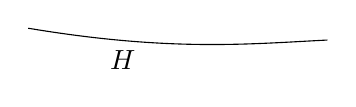
\begin{tikzpicture}[x=1cm,y=1cm]
\draw (0,0.35) .. controls (1.8,0.05) and (2.8,0.15) .. (3.8,0.2);
\node at (1.2,-0.05) {$H$};
\end{tikzpicture}}
\figure{\begin{tikzpicture}[x=1cm,y=1cm]
\draw (2.3,10.5)--(1.4,4.5)--(1.35,0);
\draw (1.55,4.5) .. controls (0.2,3.85) and (0.3,3.65) .. (1.85,4.25)
 .. controls (2.5,4.5) and (0.6,3.35) .. (1.3,3.55)
 .. controls (2.8,4) and (2.5,3.5) .. (1.05,2.5)
 .. controls (0.4,2.05) and (1.65,2.4) .. (1.7,1.8)
 .. controls (1.8,1.2) and (1.3,1) .. (1.5,0.55);
\end{tikzpicture}}

\diagram{\begin{tikzcd}
\mathbf Q_p\arrow[r,dash]&K
\end{tikzcd}}
\[
T_K(\deleted{\unsure{K}})=\prod_{K/\mathbf Q_p}G_m
\]
\margin{$\displaystyle\prod_{\unsure{o|\mathcal O}/\mathbf Z_p}\unsure{G_m}$}
\diagram{\begin{tikzcd}
{}\arrow[r]&T_{\unsure{o_K|\mathcal O_K}}\arrow[r]&\mathbf Z\arrow[r]&0
\end{tikzcd}}

\diagram{\begin{tikzcd}[column sep=small,row sep=large]
&&&&\text{Modèle de Nér. de }g_K&\\
&0\arrow[r]&g_{\unsure{0|o}}\arrow[r]&N\arrow[r]\arrow[ur,dash]&\mathbf Z_{\unsure{0|o}}\arrow[r]&0\\
\unsure{m|\text{sur}}&0\arrow[r]&g_{\unsure{0|o}}\arrow[r]\arrow[u,Rightarrow]&\widetilde N\arrow[r]\arrow[u]&\mathbf Z_{\unsure{o|0}}\arrow[r]\arrow[u]&0\\
\begin{array}{c}\unsure{m|\text{sur}}\otimes_{\unsure{o|0}}K\\\Vert\\K\end{array}
&0\arrow[r]&g_K\arrow[r]&\begin{array}{c}\widetilde N_K\\\wr\\g_K\times\mathbf Z_K\end{array}\arrow[r]&\mathbf Z_K\arrow[r]&0
\end{tikzcd}}

\diagram{\begin{tikzcd}[column sep=large,row sep=large]
0&&0\\
\mathbf Z\arrow[u]&&\mathbf Z\arrow[u]\\
T_K(\mathbf Q_p)\simeq K^*\arrow[u]&\unsure{m|\text{sur}}&{}\arrow[u]\\
\unsure{o_K|\mathcal O_K}^*\arrow[u]&&\\
0\arrow[u]&&
\end{tikzcd}}
\diagram{\begin{tikzcd}[column sep=large,row sep=large]
\Gamma(N)\arrow[r,"\sim"]&\Gamma(g)=K^*\arrow[ddl,"\pi"]\\
\Gamma(\widetilde N)\arrow[u,"\unsure{2|?}"]\arrow[d,leftrightarrow]&\\
\begin{array}{c}\Gamma(\widetilde N_K)\\\wr\\\unsure{K^*|gK^*}\times\mathbf Z\end{array}&
\end{tikzcd}}
\margin{28}
